\chapter{Research Design and Methods} \label{ch:[chapter 5 label]}

\section{Overview}
In this proposal, I have discussed the problem of search abandonment. I have noted that abandonment is partially due to search systems providing irrelevant results. This is because these systems have a weak understanding and employment of relevance. Guided by my research question, I propose a five-study research design to address this problem and improve our understanding of relevance in GIR. The relationships between studies are illustrated in figure \ref{fig:Methods_Overview}. Specifically, these studies will

\begin{enumerate}
    \item survey existing portals and record the state of faceted search,
    \item analyze a portal for user search behavior, search refinement, query topics, and latent concepts in queries that may suggest what users find relevant,
    \item analyze if and how latent concepts change with location (i.e., the location of a portal and/or datasets on a portal),
    \item modify an existing portal's search system to incorporate my findings on concept usage from the previous two studies, and
    \item evaluate the effectiveness of these modifications.
\end{enumerate}

\begin{figure}[H]
    \centering
    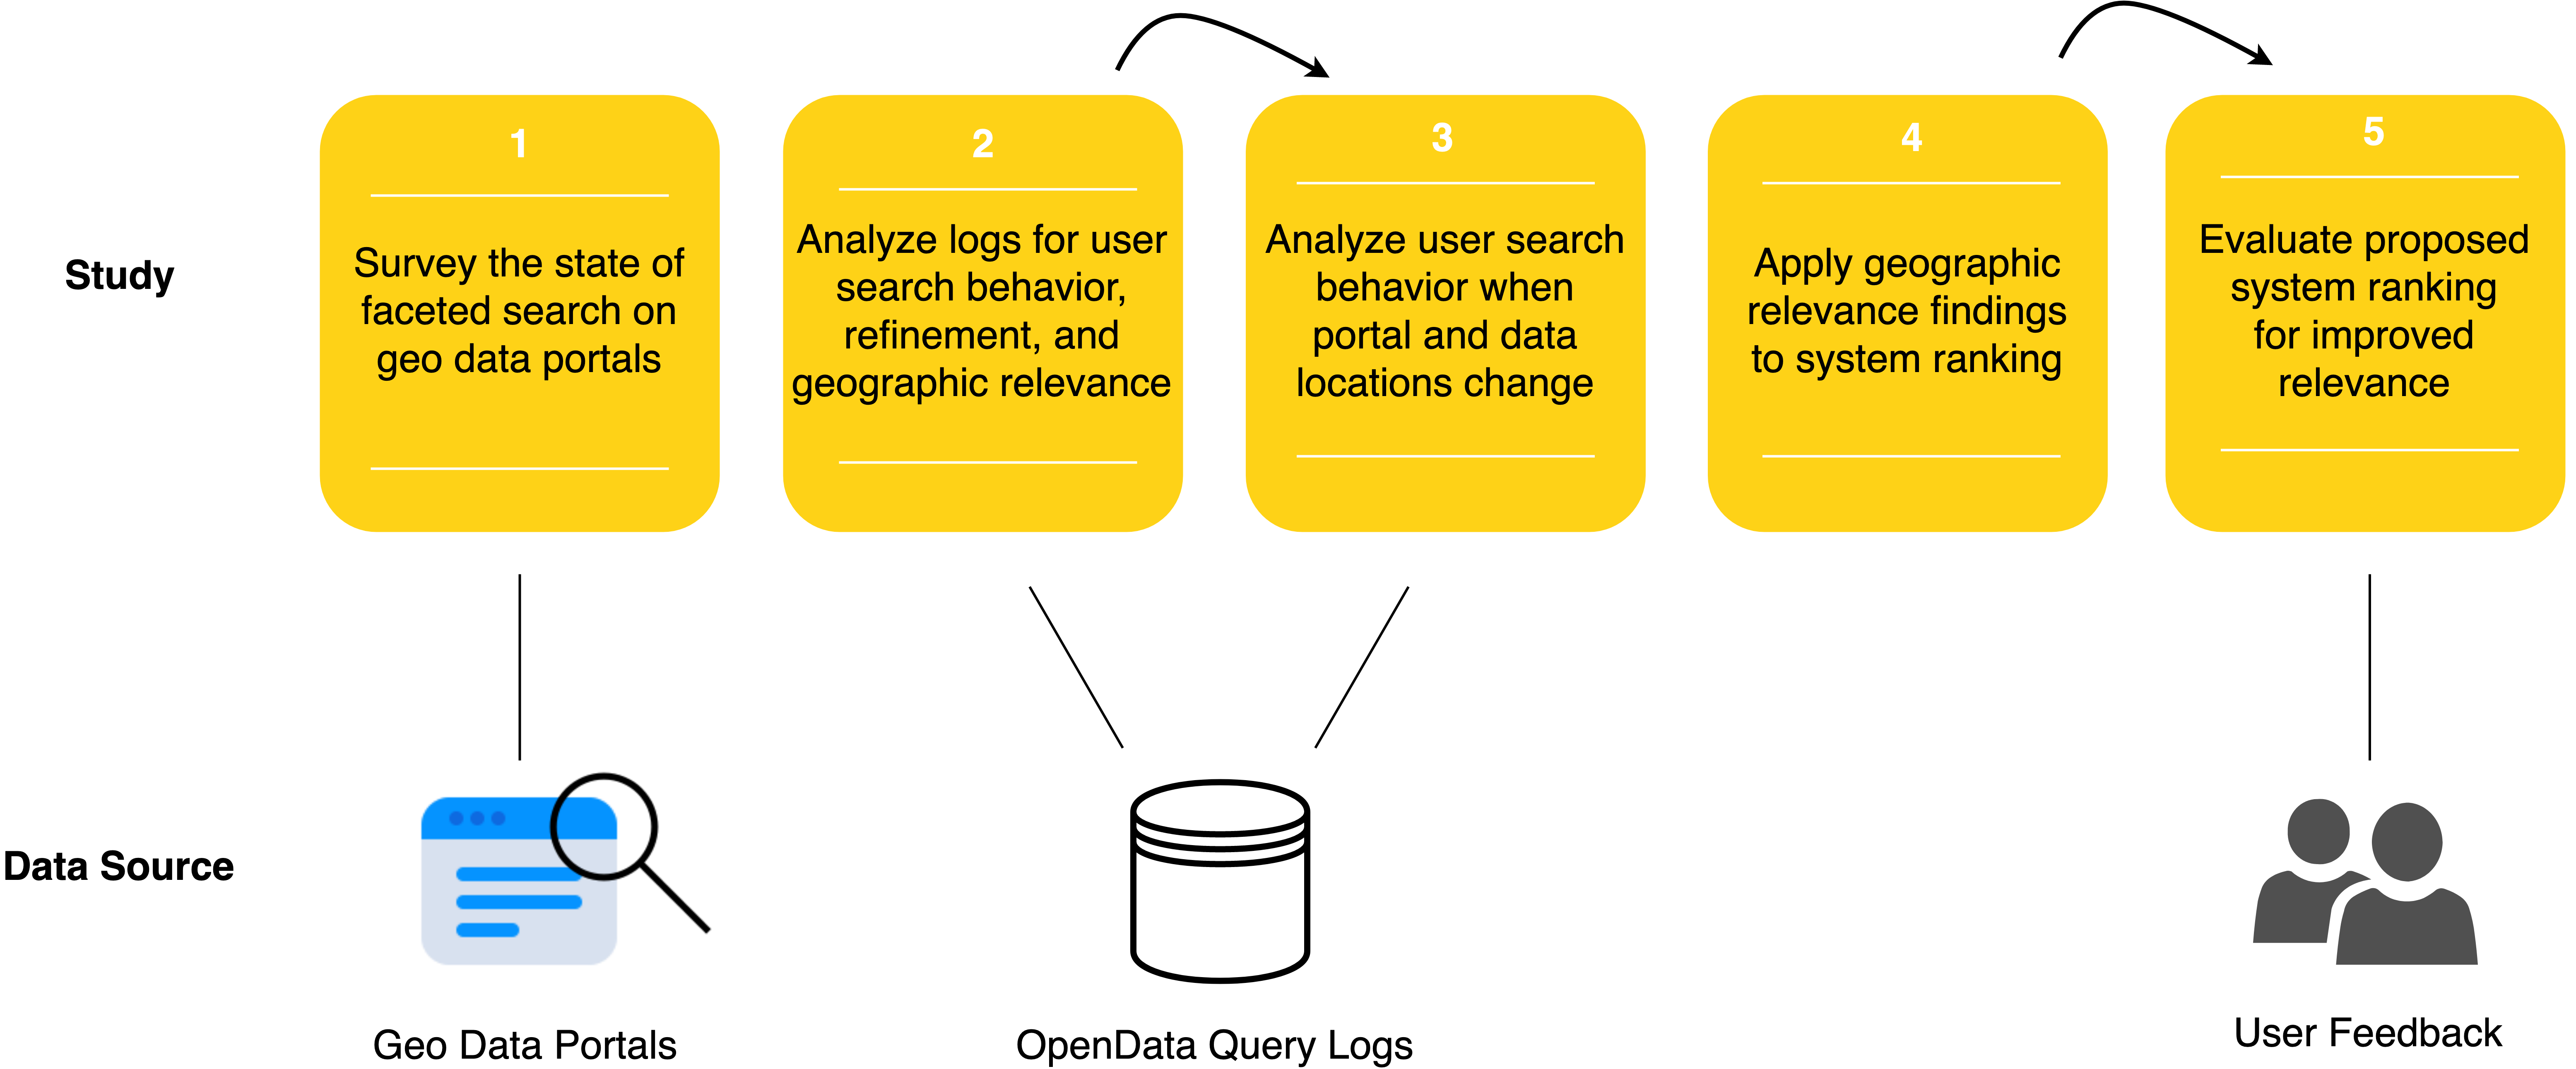
\includegraphics[width=1\textwidth]{../figures/Methods_Overview.png}
    \caption{Overview of research studies and their data sources. Studies progress by purpose including surveying the state of the art, interpreting search behavior, interpreting search behavior when location changes, applying knowledge about behavior, and evaluating the application. Arrows indicate a direct follow-up study.}
    \label{fig:Methods_Overview}
\end{figure}

\section{Surveying the State of Search Capabilities in Geospatial Data Portals}

\subsection{Study Question}
The first step to reducing search abandonment is to establish a baseline for search effectiveness. I am interested in understanding what facets users can control when they search and how search systems interpret and reason on user queries. By learning what portal users can do, I can identify gaps in their search systems. Therefore, my first research question is
\linebreak

\emph{What is the state of faceted search and ranking functions on geospatial data portals?}

\subsection{Data}
Data for this study will be collected during exploration of existing portals. I will interact with portals as a typical user and observe SERP results. Data recorded will include user-facing search facets and when documented, dataset ranking algorithms. A balanced search system strikes a balance between user control and system control. Systems with a large number of user controls dissuade serendipity, but few controls give little guidance. Portals include Esri's OpenData, data.gov, census.gov, UCSB's Alexandria Digital Library, UCSB Library's new data portal, Geoblacklight\footnote{\url{https://geoblacklight.org/}}, and several others.

\subsection{Methods}
To answer this question, I will survey the search facets of several commercial and academic portals. I will record facets such as filtering by tags, drawing a region of interest on a map, or sorting alphabetically. Figure \ref{fig:Methods_OpenData} depicts an OpenData SERP with highlights for search facets.

Most portals do not publish their search ranking functions, but many are built on open source data portals like CKAN\footnote{\url{https://ckan.org/}} and search tools like Apache Lucene\footnote{\url{https://lucene.apache.org/}}. These tools often leverage simple ranking models built on keyword similarity and \gls{tf_idf} (\acrshort{TF_IDF}). TF–IDF ranks a document highly when it has a large number of similar words to a user's query, but those words aren't common in other documents. I expect that these search systems will apply these ranking functions with minor customizations. For each portal, I will attempt several different information seeking tasks as if I were a typical user. I will simulate searching for data using specific queries for specific tasks. For example, in one scenario, I will simulate that I am a citizen who wants to reappraise their house and needs to find GIS data on parcels (to understand my property boundaries and coverage). After executing a query like "parcels", I will record the top 10 results and iteratively adjust the query to see if results change. Query adjustments will include: addition and removal of non-geographic, geographic, thematic and temporal terms, rearranging of terms, and the introduction and removal of terms indicative of the concepts that I hypothesized as being important. For example, I will add and remove spatial granularity keywords like "county" and "state", and density expressions such as "dense" or "even". Since data sparsity is likely to be an issue on some portals, I will follow several specific datasets on each portal and see how query adjustments affect their specific ranking.

\subsection{Expected Outcome}
The expected outcomes of this study will be threefold. First, this study will produce a list of observed options that affects search results on portals. This list will include all search facets and ranking criteria (and weights) when knowable. Second, this study will produce qualitative descriptions of how altering search terms affects results. Comparing queries and their responses will show if and how systems handle keywords differently. Third, this study will describe the observed deficiencies in existing systems including what queries and search facets yields irrelevant results, if any.

\begin{figure}[H]
    \centering
    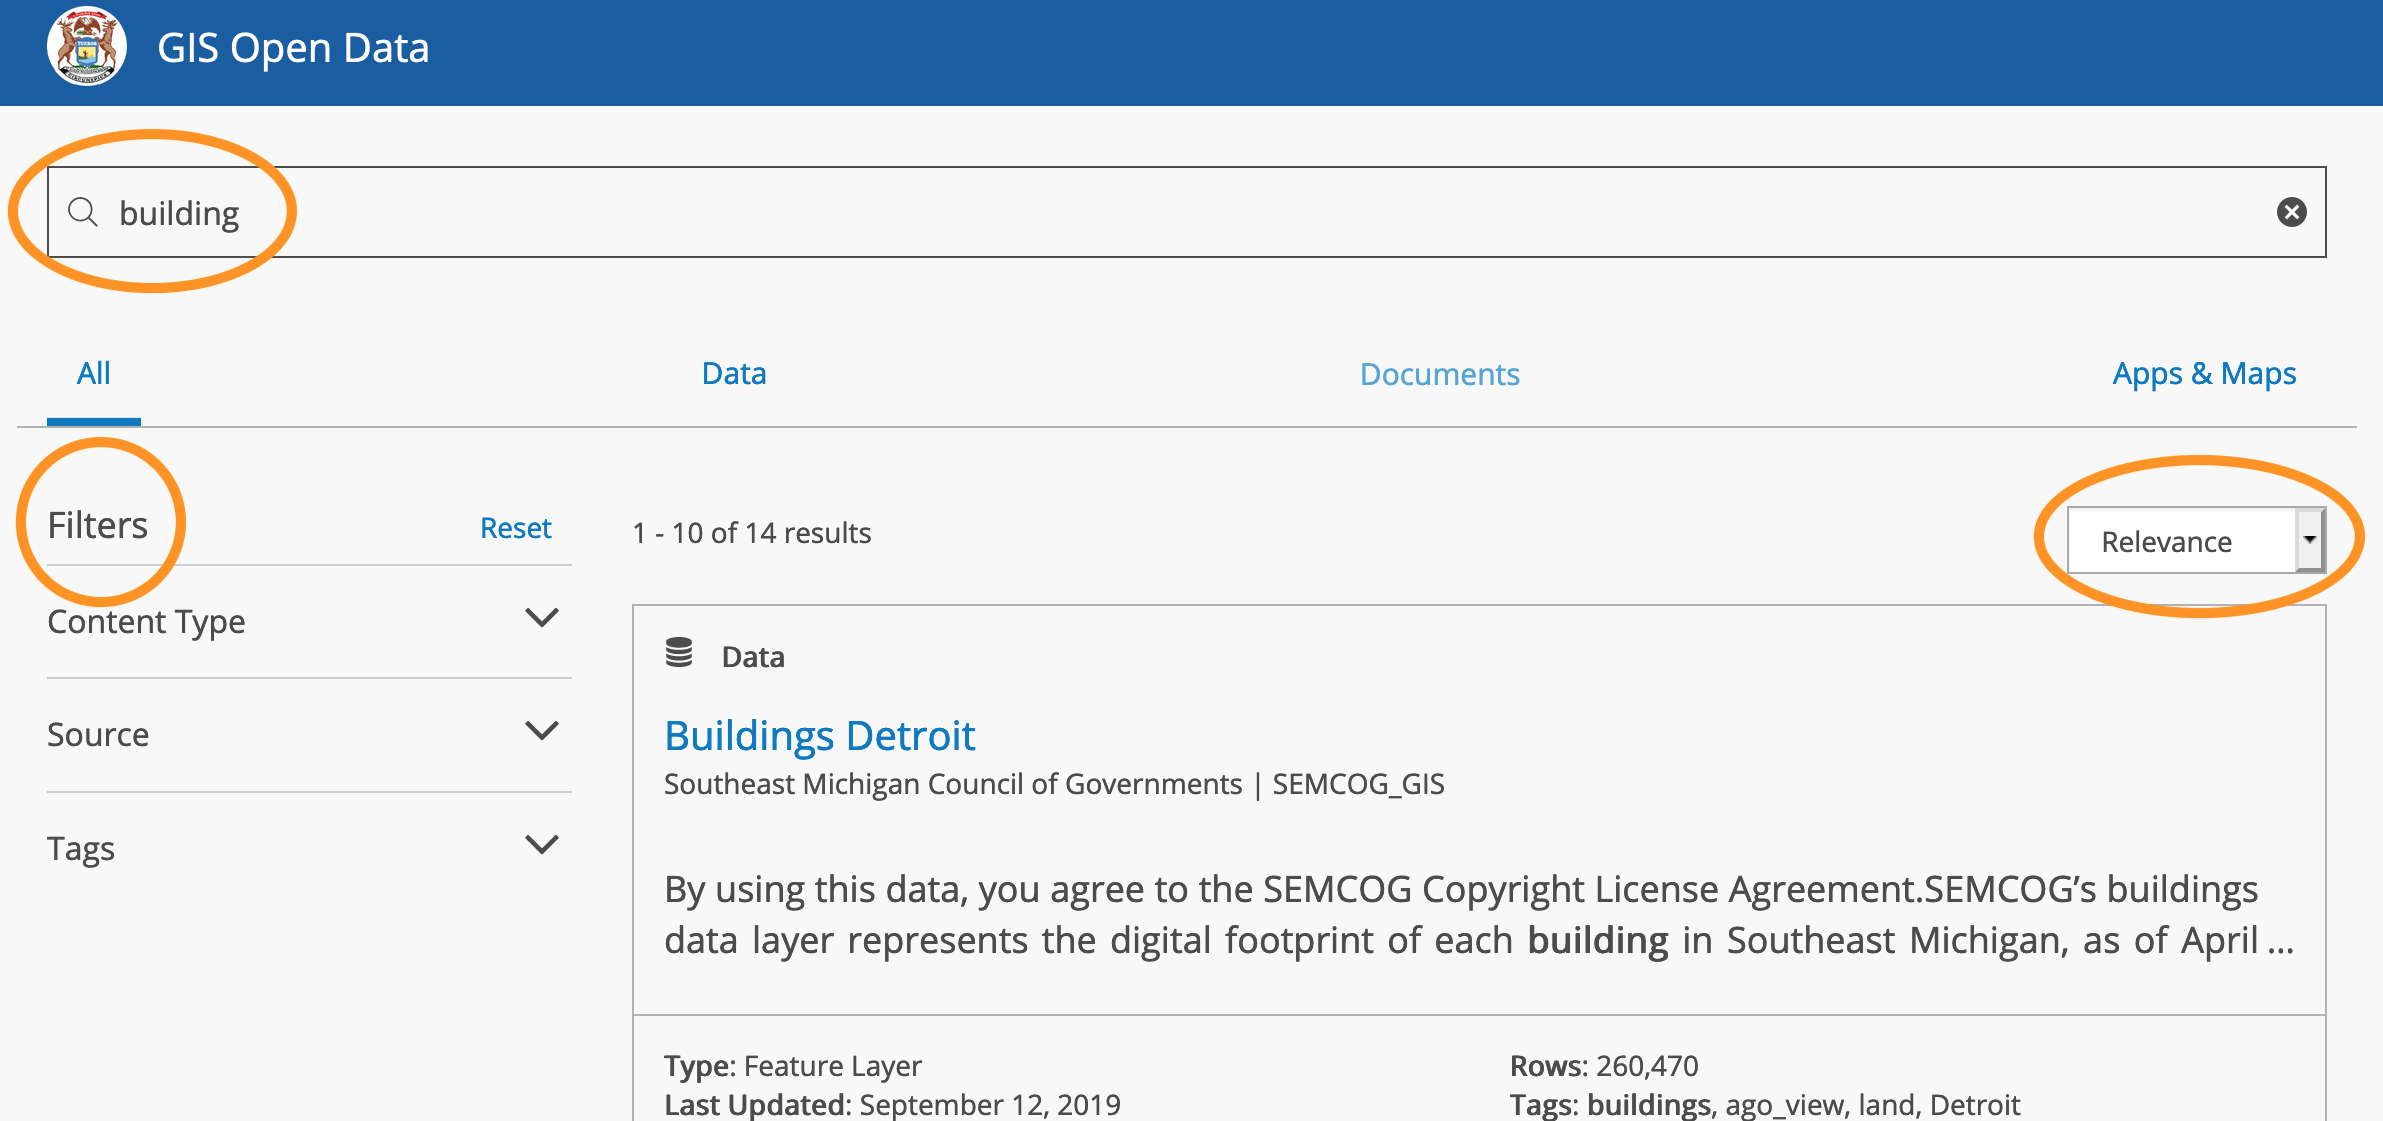
\includegraphics[width=1\textwidth]{../figures/Methods_OpenData.png}
    \caption{An example SERP from the Michigan OpenData portal. Orange highlights indicate facets that users control when searching. Surveying facets, surveying ranking functions, and observing SERP result changes from query changes are the research objectives of study 1. An ordered list of results are seen bottom right.}
    \label{fig:Methods_OpenData}
\end{figure}

\section{Extracting Concepts from User Queries to Esri OpenData Geospatial Data Portals}

\subsection{Study Question}
Surveying the state of search shows us what users can do, but what do they actually do? The next logical step is to study user search behavior. The most common approach is to analyze query logs that record system interactions. These interactions including query executions, search refinements, page clicks, navigation, downloads, dwell time, and search exits, which are behaviors indicative of relevance. Ultimately, they suggest what users commonly do, what they're asking for, where they get stuck, and what they did before they abandoned their search. Query phrases are particularly important since they are an articulation of an information need. Analyzing word and phrase usage is very important to understanding the topics and concepts that are relevant to user needs. In this study, in addition to 1) describing general search behavior and 2) search refinement patterns, I want to answer the question
\linebreak

\emph{Which concepts do people use implicitly and explicitly when searching for geospatial data, and how do they relate to search behavior and search refinement?}

% Although relevance cannot be directly quantified from query logs, certain behaviors are commonly used as relevance proxies

\subsection{Data}
In this study, I will use several related datasets. I will primarily analyze text query logs from popular portals–Esri's OpenData portals. This dataset includes over 1.5 million unique query strings, over 1 million unique search refinements, and dozens of ancillary attributes for each query string including page depth (i.e., the number of SERP results clicked), search dwell time, percentage of search abandonment, and percentage of goal conversions (i.e., percentage of downloads) among others. I have pre-processed these data and indexed them a PostgreSQL\footnote{\url{https://www.postgresql.org/}} database for use in full-text analysis. Unfortunately, due to privacy restrictions on the Google Analytics\footnote{\url{https://analytics.google.com/analytics/web/}} platform where these data originated, I am unable to extract individual search sessions. Search sessions would include what a specific user searches, clicks, and downloads. Instead, the dataset is comprised of aggregates and averages for each unique query. However, in the near future, I should have access to a second dataset called ELB logs. Once coalesced, These logs can be turned into session-like data that record what results a user clicks on following a query. These data are critical because clicks will be the foundation for constructing relevance judgements (see studies four and five for details). The last dataset contains geospatial documents, which are publicly available via on OpenData's \gls{application_programming_interface} (\acrshort{API}). All datasets will be filtered to remove non-English non-US queries and documents as a means of controlling cultural and linguistic variation in queries. These datasets combined will include the three components necessary for IR evaluation–triples of queries, documents, and relevance judgements.

\subsection{Methods}
Analyzing query logs can take dozens of different NLP data mining approaches. I will follow several classical IR and GIR approaches. Once queries are properly parsed and annotated, I will analyze the frequency, distribution, and covariance of query terms and query phrases. Then, I will identify patterns across queries, such as the frequency of specific geographic named entities, parts of speech distributions, and more. Next, semantic analysis will include identifying topics, sentiment, and explicit concepts embedded in search queries. This is conducted using robust tools for topic modeling, latent semantic analysis, and word/document embedding into vector space. Lastly, behavioral inferences are made based on the relation between findings from syntactic and semantic analysis and how a user progresses through the search process. For example, a researcher may want to know which query terms and topics most often lead to high search abandonment and/or short dwell time. Specifics for each step are as follows.

I am particularly interested in what explicit and implicit concepts users use in their queries. Therefore, I will attempt to enumerate these concepts and see how they relate to search behavior by observing two parts of my first dataset–text queries and behavior proxies (e.g, search dwell time). First, I will analyze query phrase and term usage across the entire corpus using NLP text processing techniques developed in \cite{Sanderson2007} \cite{Dittrich2015} \cite{Derungs2016} \cite{Gablasova2017} \cite{Hamzei2019b}. I will record typical IR descriptive statistics including: frequency and length of phrases, n-grams, and terms, frequency of parts of speech, and phrase dependencies. I will also attempt to model themes using the popular \gls{Latent_Dirichlet_Allocation} (\acrshort{LDA}) model and a short-text model called \gls{Dirichlet_Multinomial_Mixture} (\acrshort{GSDMM}). I will also describe general search behavior such as search trends (i.e., how OpenData usage has changed over time).

Second, I will look for the same patterns between queries. To start, I will normalize and label query terms using the same NLP methods used on the corpus and look for interactions between spatial, temporal, and thematic terms. To do this, queries are typically converted into a \gls{bag_of_words} (\acrshort{BoW}) model where word order doesn't matter but term frequency does. Then, using the \gls{vector_space_model}, feature vectors are created for the query where each feature is a BoW unigram (query term). The vector space model allows for easy similarity comparison between words and queries by calculating the cosine similarity of features. Using the vector space model, I will look for similarities between query vectors and attempt to cluster queries thematically. Since search themes widely vary, I will use a second method for comparing thematic similarity between queries. I will use ConceptNet\footnote{\url{http://conceptnet.io/}}, a semantic network built on vocabularies like Wordnet\footnote{\url{https://wordnet.princeton.edu/}}, to expand queries and reinforce findings from the vector space model. There is debate about directly applying semantic networks, but I will assume that network distance and hierarchy levels are indicative of semantic distance (within a certain threshold). I have also considered applying a geo-ontology to classify query terms, but this is not certain. Once themes are modeled, I will attempt to see how they covary with geographic and spatial terms. To do this, I will geoparse and geocode queries to label place names, addresses, and spatial qualifiers (i.e., directions like "north", relations like "inside", topology like "next to", etc.) based on pre-existing (e.g., Geonames\footnote{\url{https://www.geonames.org/}}) and custom-built databases and tools (e.g., OpenAddresses\footnote{\url{https://openaddresses.io/}}). Then, I will record if and how spatial and thematic terms covary.

Third, since query refinement is common and indicative that initial SERP results aren't relevant, I will analyze refinement patterns. Specifically I will look for query expansions, contractions, and reformulations. I will record if and how users spatially refine such as adding a zip code to an address (i.e., geocorrection) or changing place names (i.e., georeformulation), and how refinement is related to query themes, once again using ConceptNet and a threshold to set theme limits.

Fourth, based on findings from the previous three steps, I will see how query terms relate to search behavior, page progression, and abandonment. For each unique query in the corpus, there is a record for search depth, percent search exit (i.e., the rate that users leave a site after searching), search duration (i.e., the amount of time that a user spends examining results after a search), goal conversions (i.e., the rate of a goal being completed, such as downloading a dataset or making a call to the OpenData API). 

Throughout these steps, I will record the types and frequencies of explicit and implicit concepts embedded in user queries. After manually annotating these concepts for a subset of the data, I will look to see if and how they change based on the variations previously discussed (e.g., by query length, with specific query terms, after query refinement, etc.). I acknowledge that concepts can be anything and everything. I am specifically interested thematic (explicit) and latent (implicit) that could be deduced by a human reading a text query. For example, the query "2008 population density by congressional district" has several explicit and implicit concepts. The explicit concepts are a time frame (i.e., "2008"), and specific spatial unit type (i.e., the administrative unit "congressional district"). Implicit concepts give context to the themes in a query. The implicit concepts are temporal granularity (i.e., a specific year), spatial granularity (i.e., an administrative unit), and spatial configuration (i.e., density). These concepts are not pre-determined and will be expectantly debated. I believe that implicit concepts frequently found in queries that proceed search abandonment are likely neglected by the system. They should be recognized as valuable and will be incorporated into relevance ranking (see study four).

\subsection{Expected Outcome}
The expected outcome of this study will be fourfold including 
\begin{enumerate}
    \item a qualitative and quantitative description of general search patterns on Esri OpenData portals,
    \item a quantitative description of query and term frequency, query themes, and geographic and spatial term usage,
    \item a quantitative description of the types and frequencies of query refinements and geo-refinements, and how they relate to general search behavior,
    \item and a qualitative description and list of the concepts searchers use that may be indicative of what they consider relevant to their search.
\end{enumerate}

The majority of my current research is invested in this study. I have considered that this study may require being broken down into several smaller studies.

\section{Impacts of Location on Search Behavior in Search of Geographic  Datasets}

\subsection{Study Question}
This study mirrors the previous study but adds a location dimension. Previous work on map-based search suggests that the locations of users and the things and places they search for influence the themes that are searched \cite{Xiao2010}, and search systems like Google adjust for this by customizing certain search results \cite{Kliman-Silver2015}.

Since the Esri OpenData portals cover a specific location, they're each about a specific place. For example, the Michigan OpenData portal is administered by the state of Michigan and datasets roughly cover the state's footprint. So, user queries to the Michigan OpenData portal will only return datasets managed by that portal. In other words, users have local intent and portals are about a limited geography. Therefore, I want to answer the question:
\linebreak

\emph{How does local intent affect search behavior and concepts analyzed in study two?}
\linebreak

\subsection{Data}
I will use the same datasets from study two with the addition of separating queries and datasets by OpenData portal. Public OpenData datasets are accessible via a public API. Portals are at varying spatial granularity, but most are at the city level. For example, in the metadata for the Washington D.C. OpenData portal is a location represented as a bounding box of the portal's coverage.

% (a specific municipality-run portal)

\subsection{Methods}
In order to answer this question, I will examine 1000 queries issued to 50 different OpenData portals. Queries and portals will be selected using stratified random sampling to ensure diversity of portal popularity and spatial granularity. Once the queries are selected, they will be split into two groups–those that ended in success (i.e., a user downloaded a dataset) and those that ended in failure. Analysis with be conducted within group because it is difficult to compare behavior between the two. Unsuccessful search sessions are often muddier because users typically refine more and use different strategies to find relevant results.

Once the groups are formed, I will compare the results from study two between portals. Additionally, I will record differences between portals including 1) if and how georeferenced query terms, such as place names and addresses, vary in frequency and distance from a portal's coverage, and 2) if any of the results from study two differ with portal popularity and spatial granularity. I expect that theme will vary by portal but implicit concepts, especially implicit geographic concepts, will not. Depending on initial impressions of the differences between sites, if differences appear significant, I will test for statistical significance.

\subsection{Expected Outcome}
This is the shortest of the five studies. The result will be a quantitative description of how user search behavior and concepts calculated in the second study differ across selected OpenData portals. Additionally, with information about portal coverages, I can calculate how spatial relations differ between portals. The result will also include a test for correlation between the extent size of portals and the average distance of georeferenced query terms, portal popularity, and goal conversions. Further relationships may appear depending on the richness of the initial results.

\section{An Experimental Study on the Effectiveness of Introducing Concept-Based Relevance Criteria in Geographic Information Retrieval}

\subsection{Study Question}
With a better understanding of how users search and the concepts they use, the next step is to apply this knowledge to improve existing systems. Based on the results from studies two and three, I should have a list of concepts that users use when searching. These concepts may be indicative of relevant results and may be useful to include in the GIR ranking process. Therefore, I will attempt to answer the question
\linebreak

\emph{In what ways can indexing and ranking methods in GIR capture a richer notion of relevance?}
\linebreak

Note that until this point, my methods have not discussed relevance, what impacts it, and its relationship to usefulness and user satisfaction. This is because 1) I want to look at search behavior purely based on what and how users query \underline{and} because I don't yet have a relevance baseline to compare to, which will be handled in study five.

\subsection{Data}
This study does not require additional data, only a system to experiment on and some sample datasets to index and reason on, which were gathered in study three. I do not yet have access to the back end of OpenData portals to modify a cloned system, but I expect to soon. I currently have access to the ranking function that Esri uses to rank dataset results on their OpenData portals. Esri uses the Elasticsearch platform for search on OpenData portals. Their ranking algorithm is somewhat typical. It linearly combines several Elasticsearch default criteria with several custom criteria. Ranking relies on TF-IDF and is heavily keyword-based. 

\subsection{Methods}

To answer this question, I will modify an existing GIR pipeline and see if the SERP results become more relevant. Typically this incremental process is called tuning. Reconsider that general goal of tuning is to provide more relevant results to a user. Ranking, based on criteria that are used to calculate a relevance score, is an ordering of documents by how similar they match a query in vector space. Since OpenData datasets are relatively heterogeneous, I am interested in improving the precision of the results, not ensuring retrieval of all of the relevant results (i.e., recall). This study's results are evaluated in study five.

To experiment modifying a system, I will clone one existing OpenData portal and its data. Several tools that will help guide modifications including Elasticsearch's similarity computation module\footnote{\url{https://www.elastic.co/guide/en/elasticsearch/reference/current/index-modules-similarity.html}} and  ranking evaluation API\footnote{\url{https://www.elastic.co/guide/en/elasticsearch/reference/current/search-rank-eval.html}}. Modifications to the pipeline will focus primarily on incorporating the \emph{concepts} that users use. Typically, modifying criteria like this is called feature engineering. Feature engineering is where an attribute of a dataset, such as a metadata attribute, is indexed and then reasoned on by a ranking function. I will engineer features through hand tuning, not machine learning.

A newly created feature can be thought of as \emph{ranking criteria} that attempts to capture a dimension of relevance. For example, spatial granularity is one potential feature. To create a feature for spatial granularity, datasets will be compared with curated administrative datasets such as the US-wide block group, census tract, county, and state Census TIGER/Line shapefiles. If a dataset has a spatial granularity at the county level, an indexed attribute will created for the dataset and assigned a value of 3 based on county's hierarchical position in the Getty Thesaurus of Geographic Names. Spatial granularity of the dataset can then be reasoned on and compared with the spatial granularity in a query when present.

% Incorporating findings means that the GIR pipeline will ingest and reason on new criteria for ranking. These criteria are meant to capture relevance as best as possible. My approach is experimental and for the moment, improvements will be anecdotal. 
% Then, I will test if incorporating the findings from the second and third study into the portal's ranking algorithm improves results.

Modifications to the ranking function will start out as a simple linear combination of existing features with one or two additional features. However, there will likely be other important concepts such as those in my hypothesis. There are no exact rules on how to create features, so I will likely have to hand tune classes for feature values. This is a typical process for tuning a ranking algorithm. Once a feature is indexed, it can be reasoned on as criteria during ranking. These criteria can be weighted, boosted, and then combined with other criteria like keyword similarity.

Note that these methods are rapidly developing. Hand tuning is difficult, but at the moment, I do not plan to use any machine learning models for improving ranking. This is because I do not yet know how dramatically feature engineering will change ranking. More complex models, such as the \gls{learn_to_rank} (which uses \gls{support_vector_machines} to predict ranking) require a more mature understanding of the effects of tuning and the target data. Also, I will also not yet use language models which reverse engineer queries based on document details (suggesting what criteria can be used for reasoning).

\subsection{Expected Outcome}
The expected outcome of this study is twofold including
\begin{enumerate}
    \item a new indexing pipeline for OpenData datasets (and potentially specific embedded data features), and 
    \item an expanded ranking algorithm that incorporates new criteria created through feature engineering
\end{enumerate}

Since result improvements will be based on anecdotal evidence, it is likely that both of these outcomes could vary spatial granularity based on my domain knowledge. However, in the next study, these outcomes will be methodically testing using standard evaluation methods.

\section{Evaluating the Effectiveness of Adding Concepts in Queries as Relevance Criteria into a GIR Ranking Function}

\subsection{Study Question}
To test the effectiveness of modifications made in study four, the modifications will be subject to evaluation. I will attempt to answer the question
\linebreak

\emph{Will adding the proposed concepts as relevance criteria improve ranking of geographic datasets as measured by several offline and online measures?}
\linebreak

\subsection{Data}
This evaluation framework will be comprised of at least two and possibly three evaluation methods highlighted in figure \ref{fig:Methods_Evaluation}. These methods will be both \emph{online} (using a live search environment) and \emph{offline} (using a test collection). First, I will create a custom-built test collection. This will be time consuming initially but then automated. The test collection will be constructed using the ELB logs and will comprise queries-document-relevance judgement triples. The ELB logs record all requests made to the OpenData servers, passing through the Elasticsearch engine. Therefore, I will be able to recreate (somewhat superficial) search sessions that are breadcrumbs of a user's search progression. A typical progression will probably resemble \emph{query}, \emph{click SERP result}, \emph{return to SERP}, \emph{click second result}, \emph{download result or exit search}. Explicit relevance judgements are difficult and costly to acquire. They require experts manually annotating the relevance of each SERP result for a set of queries. Instead, I will calculate an \emph{implicit} relevance judgement called \emph{pseudo relevance feedback}. Note that this test collection may be made in a prior study for prior analysis.

Second, I will gather data on click deviation during A/B testing. These data will show how user clicks (i.e., which SERP results they click and/or download) differ between two systems, a control system and a modified system. The methods second describes how I will collect and use these data.

\subsection{Methods}
Evaluating IR systems is a difficult and often confusing process. There is a lot of noise in query logs caused by variability in user preferences and queries. Therefore, most researchers conducting IR evaluation use the \emph{offline} system-view by examining a pre-defined test collection and calculating measures like precision, recall, MAP and NGDC. I will loosely follow this approach because strict adherence would require that I collect explicit relevance feedback. As previously mentioned, explicit relevance feedback is both expensive and difficult to do properly hence why most IR research uses benchmark test collections. Instead, I will conduct an offline evaluation but using \emph{pseudo relevance feedback}. It is an indirect feedback that is a well proven replacement for explicit relevance feedback \cite{Manning2008}. Instead of manually annotating relevance judgements, predetermined top \emph{k} documents are considered relevant. Then, a query is expanded to incorporate terms in the top ranked documents and new vector space classifications are drawn using the \gls{Rocchio_classification} algorithm. Last, typical ranking methods like TF-IDF and system-view evaluation measures like precision and recall can be recalculated.

The next step is to test for improvement. Using several subsets of the test collection (e.g., records to one OpenData portal or records with popular queries), I will compare precision, recall, NGDC, and MAP scores between the existing and modified systems and then test for statistical significance. I will focus on NGDC at ranks 1,3,and 5, and MAP. Note that based on my understanding, there are limitations to this approach and it may not be explanatory. I will continue to gather evidence on the effects of pseudo relevance feedback and how evaluation must be altered to account for it.

Studies suggest that online evaluations are a better way to assess not just relevance but usefulness and user satisfaction \cite{Hofmann2016} \cite{Zhang2018} \cite{Chen2017}. Therefore, I will also conduct online evaluations. To do this, I will use a combination of A/B testing and click-through data to compare user behavior between the existing and modified systems. First I will stand up a live version of the modified system. This "\emph{B}" system will likely be run by Esri but may need to be run in a controlled experimental environment at UCSB. Average users who issue queries to OpenData will either be sent to the existing system or the modified system. Several behaviors will be recorded including \gls{click_deviation} (when users select a result that isn't the top result suggesting that it is more relevant), search successes (downloading a dataset), and search failure (leaving without a success or abandoning the session). These are user \emph{preferences} typically seen as proxies for relevance judgements.

Differences between systems can only be compared when either search tasks or queries are the same. Since queries are frequently issued to OpenData portals (and many queries have a high frequency), I expect that I can select a subset of congruent queries between the A and B systems without needing to supervise a controlled search task experiment. After collecting query logs containing behaviors like click deviations, I will look to see if click deviations decrease and if they is significant. I will also look to see if and how search success and failure rates change, and if they vary by portal.

Time permitting, I will use findings from the online evaluation to revisit and improve relevance judgements for offline evaluation. Click deviations can also be used to construct non-binary relevance judgements. For example, if a user clicks the third result, that document's relevance score can be boosted. Downloads could boost the score even more, and search failures can reduce the score of all the results. After collecting enough judgements for a small set of queries, offline evaluations can be conducted again and results can be compared to the evaluation measure scores when using only pseudo relevance feedback.

% A download will mean that the document downloaded is relevant and that the search session is successful. Alternatively, search exits will mean that the datasets are not relevant. For example, if a query is issued with no refinements and results in a downloaded dataset, this can be considered a successful search session. If a user refines their search multiple times and doesn't download a dataset, this is an example of an unsuccessful session. I will separate and compare the results between successful and unsuccessful sessions. As mentioned previously, this method will be used for creating relevance judgements until I have access to the ELB logs.

% Results will be more meaningful once I curate the ELB logs because it more closely resembles search sessions where a user executes a query, clicks on certain results, and ultimately downloads a dataset or abandons the session. In this case, clicks will be used in conjunction with goal conversions to create relevance judgements. Clicks are highly variable and literature suggests that a click does not mean that a result is relevant. However, a click, particularly if it isn't to the top result, indicates preference and that the result is relatively more valuable than the top result. Therefore, clicks can be used in a probabilistic model for calculating relevance scores. Furthermore, clicks can be combined with more concrete relevance proxies, such as goal conversions discussed earlier. It is likely that this method for determining relevance judgements will be improved before this study is complete. Ultimately, the ELB logs will be used to create a test collection of query–document–relevance judgement triples. In theory, this test collection, were it to be made public, would be useful for future GIR evaluations.

%  I expect that there will be several improvements to the ranking process. The first is that precision and recall will increase. I also expect that normalized discounted cumulative gain (NDCG), a popular metric for top result ranking quality, will significantly improve since Esri's OpenData ranking of the top 10 results is currently heavily keyword based. To measure this, I will 1) compare evaluation metrics (i.e., precision, recall, NGDC) before and after ranking adjustments, and (time permitting) 2) compare search behavior before and after adjustments. I will use abandonment (i.e., exit rate), depth, and goal conversions as indicators for a successful or unsuccessful search session. Note, these events (exit rate, depth, goal conversion) are only proxies for relevance, but are used widely in the literature. *Using Esri's existing Hub platform and with the assistance of Dan Montello, I design a modified OpenData portal to record user behavior and survey users to ask what they were searching for and how the results between the two systems compare

\subsection{Expected Outcome}
As the last study in my research, I expect to produce two conclusions: 1) whether or not concepts I believe are important (e.g., spatial granularity) are indeed important to users, and 2) if and how evaluation results answer my research question, specifically if incorporating the concepts mentioned herein improve ranking. As far as results, I expect that, if conducted correctly, MAP and NGDC at rank 1 and 3 will significantly improve in the modified system. I also expect that search failure will decrease, but I am uncertain if it will be significant. Development-wise, I expect to produce a reusable test collection of geospatial query-document-relevance judgements. I also expect that my findings throughout this research, especially from the last two studies, will be directly used in Esri's OpenData search product.

\begin{figure}[H]
    \centering
    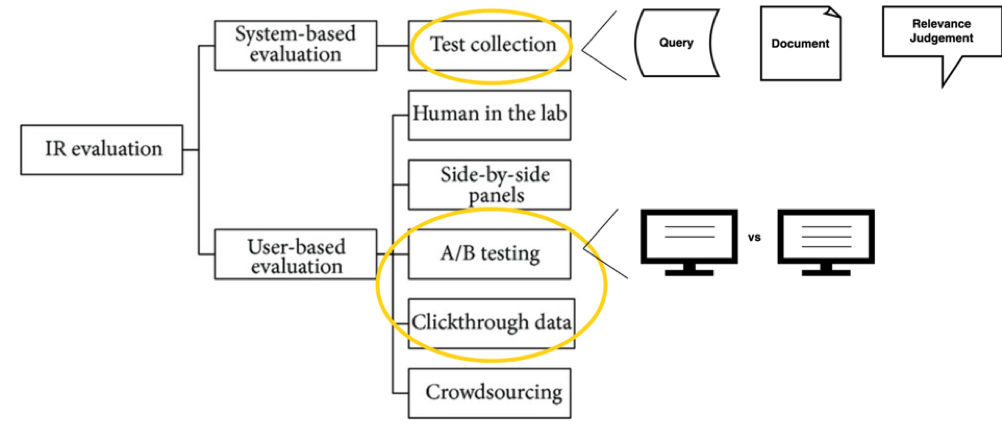
\includegraphics[width=1\textwidth]{../figures/Methods_Evaluation.png}
    \caption{Classification of IR evaluation approaches adapted from \cite{Samimi2014}. Yellow highlights indicate the evaluation approaches used in this study. A test collection comprises a query, document, and relevance judgement for each query-document and compares their behavior. I will also add an option for self-reported relevance on each SERP result. Click-through data, parsed from query logs in study 2, will be used to cross-reference A/B testing results.}
    \label{fig:Methods_Evaluation}
\end{figure}